%
% This is the LaTeX template file for lecture notes for CS294-8,
% Computational Biology for Computer Scientists.  When preparing 
% LaTeX notes for this class, please use this template.
%
% To familiarize yourself with this template, the body contains
% some examples of its use.  Look them over.  Then you can
% run LaTeX on this file.  After you have LaTeXed this file then
% you can look over the result either by printing it out with
% dvips or using xdvi.
%
% This template is based on the template for Prof. Sinclair's CS 270.

\documentclass[twoside]{article}
\usepackage{graphics}
\usepackage{amsmath}
\usepackage{amssymb}
\usepackage{hyperref}
\usepackage{IEEEtrantools}
\usepackage{graphicx}
\setlength{\oddsidemargin}{0.25 in}
\setlength{\evensidemargin}{-0.25 in}
\setlength{\topmargin}{-0.6 in}
\setlength{\textwidth}{6.5 in}
\setlength{\textheight}{8.5 in}
\setlength{\headsep}{0.75 in}
\setlength{\parindent}{0 in}
\setlength{\parskip}{0.1 in}
\usepackage[makeroom]{cancel}
%
% The following commands set up the lecnum (lecture number)
% counter and make various numbering schemes work relative
% to the lecture number.
%
\newcounter{lecnum}
\renewcommand{\thepage}{\thelecnum-\arabic{page}}
\renewcommand{\thesection}{\thelecnum.\arabic{section}}
\renewcommand{\theequation}{\thelecnum.\arabic{equation}}
\renewcommand{\thefigure}{\thelecnum.\arabic{figure}}
\renewcommand{\thetable}{\thelecnum.\arabic{table}}

%
% The following macro is used to generate the header.
%
\newcommand{\lecture}[4]{
   \pagestyle{myheadings}
   \thispagestyle{plain}
   \newpage
   \setcounter{lecnum}{#1}
   \setcounter{page}{1}
   \noindent
   \begin{center}
   \framebox{
      \vbox{\vspace{2mm}
    \hbox to 6.28in { {\bf CMPUT 652: Reinforcement Learning with Robots
                        \hfill Fall 2019} }
       \vspace{4mm}
       \hbox to 6.28in { {\Large \hfill Lecture #1: #2  \hfill} }
       \vspace{2mm}
       \hbox to 6.28in { {\it Instructor: #3 \hfill Scribe: #4} }
      \vspace{2mm}}
   }
   \end{center}
   \markboth{Lecture #1: #2}{Lecture #1: #2}
   {\bf Disclaimer}: {\it These notes have not been subjected to the
   usual scrutiny reserved for formal publications.  They may be distributed
   outside this class only with the permission of the Instructor.}
   \vspace*{4mm}
}

%
% Convention for citations is authors' initials followed by the year.
% For example, to cite a paper by Leighton and Maggs you would type
% \cite{LM89}, and to cite a paper by Strassen you would type \cite{S69}.
% (To avoid bibliography problems, for now we redefine the \cite command.)
% Also commands that create a suitable format for the reference list.

%% This has been commented by Dhawal
% \renewcommand{\cite}[1]{[#1]}
% \def\beginrefs{\begin{list}%
%         {[\arabic{equation}]}{\usecounter{equation}
%          \setlength{\leftmargin}{2.0truecm}\setlength{\labelsep}{0.4truecm}%
%          \setlength{\labelwidth}{1.6truecm}}}
% \def\endrefs{\end{list}}
% \def\bibentry#1{\item[\hbox{[#1]}]}

%Use this command for a figure; it puts a figure in wherever you want it.
%usage: \fig{NUMBER}{SPACE-IN-INCHES}{CAPTION}
\newcommand{\fig}[3]{
			\vspace{#2}
			\begin{center}
			Figure \thelecnum.#1:~#3
			\end{center}
	}
% Use these for theorems, lemmas, proofs, etc.
\newtheorem{theorem}{Theorem}[lecnum]
\newtheorem{lemma}[theorem]{Lemma}
\newtheorem{proposition}[theorem]{Proposition}
\newtheorem{claim}[theorem]{Claim}
\newtheorem{corollary}[theorem]{Corollary}
\newtheorem{definition}[theorem]{Definition}
\newenvironment{proof}{{\bf Proof:}}{\hfill\rule{2mm}{2mm}}

% **** IF YOU WANT TO DEFINE ADDITIONAL MACROS FOR YOURSELF, PUT THEM HERE:

%%===========================================================================
%% defining the expectation operator
%%---------------------------------------------------------------------------
\DeclareMathOperator{\E}{\mathbb{E}}
\DeclareMathOperator{\Real}{\mathbb{R}}
\DeclareMathOperator{\real}{\mathbb{R}}
\DeclareMathOperator{\xvec}{\textbf{x}}
% \DeclareMathOperator{\thetagd}{\theta^{GD}}
% \DeclareMathOperator{\rv}{X} % define random variable 
% \DeclareMathOperator{\sc}{} %
% \DeclareMathOperator{}{} %
% \DeclareMathOperator{}{} %
% \DeclareMathOperator{}{} %

% \DeclareMathOperator{}{}
%%===========================================================================

\begin{document}
%FILL IN THE RIGHT INFO.
%\lecture{**LECTURE-NUMBER**}{**DATE**}{**LECTURER**}{**SCRIBE**}
\lecture{4}{September 12}{Rupam Mahmood}{Dhawal Gupta}
%\footnotetext{These notes are partially based on those of Nigel Mansell.}

% **** YOUR NOTES GO HERE:

% Some general latex examples and examples making use of the
% macros follow.  
%**** IN GENERAL, BE BRIEF. LONG SCRIBE NOTES, NO MATTER HOW WELL WRITTEN,
%**** ARE NEVER READ BY ANYBODY.

\section{Discussion: Last Lecture}
The last lecture discussed the formulation and optimization of the objective function, along with the methods of averaging, gradient descent and stochastic gradient descent as well as the bias-variance trade-off and bias and variance in using the square distance for Gaussian parameter estimation.

\section{Notation}

The notation that we are going to follow in these notes have been borrowed from \cite{sutton2018reinforcement} and is described below.
\bigskip\noindent
\begin{tabbing}
\=~~~~~~~~~~~~~~~~~~  \= \kill
\>$X$   \> Random variables (scalar)\\
\>$x$    \> Values of random variables or scalar functions\\
\>$\textbf{x} $    \> Quantities required to be real-valued coloumn vectors (even random variables)\\
\>$\textbf{X}$    \> Matrices\\
\>$\textbf{X}^T, \textbf{x}^T$    \> The transpose of a matrix or vector\\
\>$[\textbf{x}]_i$    \> The \textit{i}-th element of the vector.\\
\>$[\textbf{X}]_{i:}$    \> The \textit{i}-th row of the matrix. A row vector\\
\>$[\textbf{X}]_{:j}$    \> The \textit{j}-th column of the matrix. A column vector\\
\>$[\textbf{X}]_{ij}$    \> The \textit{i,j}-th element of the matrix.\\
\>$\textbf{x}_t$    \> The vector at time t\\
\>$X_t$    \> The random variable at time t\\



\end{tabbing}

\section{Linear Function Approximation}
We will be using the mean squared error as the objective function for the approximation of the parameter in the case where our modelled function $f$ is a linear model.
\begin{equation}\label{eq:linear_model}
    f(\textbf{x}) = \textbf{x}^T\theta
\end{equation} 
where $\textbf{x},\theta \in \real^p$, p is the number of features in our input. Y is the output variable which takes in real value, i.e. $Y \in \real$

We assume that both $(\textbf{x},Y)$ are sampled from a joint probability distribution that is not know, but we have access to the samples from that probability distribution i.e. $\{(\textbf{x}_i,Y_i)\}_{i =0}^{t} \sim P(\textbf{x},Y)$ also reffered as a training data set. 

\subsection{Exact vs. Sample-based MSE objectives}
Here we list the different forms of the objective function for the cases of exact and sampled based estimates of the objective function.


The exact form of the squared error loss function can also written as $\mathcal{V}(\theta)$ i.e.
\begin{equation}\label{eq:MSE_exact}
    \mathcal{V}(\theta) = MSE = \E[(Y - \textbf{x}^T\theta)^2]
\end{equation}

The sample based objective function for dataset $\{ (\textbf{x}_i, Y_i)\}_{i = 1}^{t}$ : 
\begin{equation}\label{eq:MSE_sample}
    \hat{MSE} = \dfrac{1}{t}\sum_{i = 1}^{t}(Y_i - \textbf{x}_i^T\theta)^2
\end{equation}

And the squared error at time T = t, is written as 
\begin{equation}
    SE_t  = (Y_t - \textbf{x}_t^T\theta)^2
\end{equation}

By the law of large numbers as $t \rightarrow \infty$, $\hat{MSE} \rightarrow MSE$ given i.i.d sampling of $(\textbf{x}_i, Y_i) \sim P(\textbf{x}, Y)$.

\subsection{Optimization of the Objective function}
We will be going through the different approaches to optimizaiton of the objective functions starting from the one step , exact optimization procedure moving onto\textbf{ Gradient Descent} (GD) and \textbf{Stochastic Gradient Descent} (SGD) finding the optimal $\theta$ i.e. $\theta^*$ for the linear model \ref{eq:linear_model}.
Here we are taking the expectation over $(\textbf{x}, Y)$.


Equations \ref{der:MSE_exact} provides an exact optimization process in the case of availability of Expectation of different variables.
\begin{equation}\label{der:MSE_exact}
    \begin{split}
        \mathcal{V}(\theta) &= \E[(\underset{1 \times 1}{Y} - \underset{1 \times p}{\textbf{x}}^T\underset{p \times 1}{\theta})^2] \text{  (from \ref{eq:MSE_exact})}\\
        &= \E[(Y - \textbf{x}^T\theta)^T(Y - \textbf{x}^T\theta)]\\
        &= \E[ \underset{1 \times 1}{Y^2} + \underset{1 \times p}{\theta^T}\underset{p \times 1}{\textbf{x}}\underset{1 \times p}{\textbf{x}^T}\underset{p \times 1}{\theta} - 2\underset{1 \times p}{\theta^T}\underset{p \times 1}{\textbf{x}}\underset{1 \times 1}{Y}]\\
        &= \E[Y^2] + \theta^T\E[\textbf{x}\textbf{x}^T]\theta - 2\theta^T\E[\textbf{x}Y]\\
        \text{Doing the following substitution } \textbf{A} &= \E[\textbf{x}\textbf{x}^T], \textbf{b} = \E[\textbf{x}Y], c = \E[Y^2] \text{we get..}\\
        &= \theta^T\textbf{A}\theta - 2\theta^T\textbf{b} + c\\
        \text{taking } & \text{the gradient}\\
        \nabla_\theta\mathcal{V}(\theta) &= 2 \textbf{A} \theta - 2 \textbf{b}\\
        \text{which}&\text{ gives us }\\
        \theta^* &= \textbf{A}^{-1}\textbf{b} 
    \end{split}
\end{equation}

So \ref{der:MSE_exact} gives us the following after putting the values of $\textbf{A}, \textbf{b}, c$
\begin{equation}
    \theta^* = \E[\textbf{x}\textbf{x}^T]^{-1}\E[\textbf{x}Y]
\end{equation}

We can extend the above result to generalize to the sample based method i.e. placing this for \ref{eq:MSE_sample}\footnote{I have tried to show a separate proof of this, which can be easily inferred from \ref{der:MSE_exact} as well}
\begin{equation}\label{eq:MSE_exact_solution}
     \theta_{t+1} = (\dfrac{1}{t}\sum_{i=1}^{t}\textbf{x}_i\textbf{x}_i^T)^{-1}(\dfrac{1}{t}\sum_{i=1}^{t}\textbf{x}_i Y_i)
\end{equation}

Writing the step wise update rule for GD i.e.
\begin{equation}
\begin{split}
    \theta_{t+1}^{GD} &= \theta_{t}^{GD} - \alpha_t \nabla_{\theta_t^{GD}}\mathcal{V}(\theta_t^{GD})\\
    \theta_{t+1}^{GD} &= \theta_{t}^{GD} - 2\alpha_t(\textbf{A}\theta_t^{GD} - \textbf{b}) \text{( from \ref{der:MSE_exact})}
    \end{split}
\end{equation}

% @dhawgupta  : In the expression of the stepwise update rule for gradient descent, is the value of A and b empriically decided, i.e. , do we put it as A_t, and b_t, where the A_t is either the sum of 0 to t, or only in terms of the last value of T , I was not able to find an iterative version for A_t and b_t


Similarly this can be written for the case of SGD i.e.
\begin{equation}\label{eq:gradient_descent}
\begin{split}
    \theta_{t+1} &= \theta_t - \alpha_t\nabla_{\theta_t}(Y_t - \theta_t^T\textbf{x}_t)^2\\
    \theta_{t+1} &= \theta_t + 2\alpha_t(Y_t - \theta_t^T\textbf{x}_t)\textbf{x}_t
\end{split}
\end{equation}

\textbf{Note} : We can try to write these formulation of \ref{eq:MSE_sample} in a time based manner as well, I tried but I am not able to figure one out, just similar to the case of moving average

% @dhawgupta : So in the slides, there is pointe raobut Least Squared Methods, unbiasednedd and consistency, neeed to dsicuss that

\subsection{Gradient Descent Method and Convergence}
Below we expand the $\theta_{t+1}^{GD}$ term to understand the behaviour of convergence.

\begin{equation}
    \begin{split}
        \theta_{t+1}^{GD} =& (I - \alpha \textbf{A})\theta_t^{GD} + \alpha \textbf{b }\text{   ( \textbf{A}, \textbf{b} from \ref{der:MSE_exact} \& $\alpha_t = \dfrac{\alpha}{2}$ )}\\
        =& \alpha \textbf{b} + (I - \alpha \textbf{A})[(I - \alpha \textbf{A})\theta_{t-1}^{GD} + \alpha \textbf{b}]\\
        =& \alpha \textbf{b} + \alpha (I - \alpha \textbf{A}) \textbf{b} + (I - \alpha \textbf{A})^2\theta_{t-1}^{GD}\\
        =& \alpha[I + (I - \alpha \textbf{A}) + (I - \alpha \textbf{A})^2 + ... + (I - \alpha \textbf{A})^t]b + (I - \alpha \textbf{A})^{t+1}\theta_{0}^{GD}\\
        \text{ Using the } & \text{Geometric Series Summation}\\
        =& \cancel{\alpha} (\cancel{I} - \cancel{I} + \cancel{\alpha} \textbf{A} )^{-1}[I - (I - \alpha \textbf{A} )^{t+1}]b + (I - \alpha \textbf{A})^{t+1}\theta_{0}^{GD}\\
        =&\textbf{ A}^{-1}[I - (I - \alpha \textbf{A} )^{t+1}]\textbf{\textbf{b}} + (I - \alpha \textbf{A})^{t+1}\theta_{0}^{GD}\\
    \end{split}
\end{equation}

This series is convergent as $(I - \alpha \textbf{A})^{t}$ goes to zero for the following conditions  
\begin{equation}\label{eq:meta_condition}
    \rho( I - \alpha \textbf{A}) < 1
\end{equation}

where the spectral radius $\rho(\textbf{B})$ for a matrix $\textbf{B}$ is defined as 
\begin{equation}\label{eq:def_spectral}
    \rho(\textbf{B}) = \underset{i}{max}|eig_i(\textbf{B})|
\end{equation}

Hence for \ref{eq:meta_condition} we need the following to hold 
\begin{equation}
    Re({eig}_i \textbf{A}) > 0
\end{equation}

So in the limit of $t\rightarrow \infty$ the value converges to $\textbf{A}^{-1}\textbf{b} = \theta^*$, hence telling us that the bias goes to zero along with the more no of examples observed.

\begin{equation}
    \underset{t \rightarrow \infty}{\lim} \theta_t^{GD} = \textbf{A}^{-1}\textbf{b}
\end{equation}

As $\textbf{A}$ is symmetric matrix, all eigen values of $\textbf{A}$ are Real.

\textbf{Note}: This part has been added by scriber (need to check validity) : 
Finding the conditions on eigen values of matrix $\textbf{A}$ i.e. $\lambda_a$

taking $\textbf{x}$ as the eigen vector and $\lambda$ as the corresponding eigen value for $(I - \alpha \textbf{A})$

\begin{equation}
    \begin{split}
        (I - \alpha \textbf{A})\textbf{x} &= \lambda \textbf{x}\\
        (1 - \lambda)\textbf{x} &= \alpha \textbf{A} \textbf{x}\\
        \dfrac{(1 - \lambda)}{\alpha}\textbf{x} &= \textbf{A}\textbf{x}\\
        \text{from above it seems that $\textbf{x}$ is eigen vector}& \text{ for $A$ where $A$ has eigen values $\dfrac{(1-\lambda)}{\alpha}$ }\\
        \dfrac{(1-\lambda)}{\alpha} &= \lambda_a\\
    \end{split}
\end{equation}
\begin{equation}\label{eq:lambda_in_lambda_a}
     \lambda = (1-\alpha \lambda_a)
\end{equation}

From \ref{eq:lambda_in_lambda_a} we can get the conditions that need to be applied on top of the eigenvalues of $\textbf{A}$ i.e. $\lambda_a$.

From \ref{eq:meta_condition} and \ref{eq:def_spectral} we get the following conditions. As $\lambda_a$ is always real we dont need to worry about complex eigenvalues.
We have that 
\begin{equation}
    \begin{split}
    |\lambda| &< 1 \text{ (for all $\lambda$) }\\
    |(1 - \alpha \lambda_a) | &< 1 \text{  (from \ref{eq:lambda_in_lambda_a})}
    \end{split}
\end{equation}

Case 1: $\lambda_a \leq \dfrac{1}{\alpha}$
\begin{equation}
    \begin{split}
        (1 - \alpha \lambda_a) &< 1\\
        \lambda_a & > 0
    \end{split}
\end{equation}
This gives us 
\begin{equation}\label{eq:condition}
    0 < \lambda_a \leq \dfrac{1}{\alpha}
\end{equation}

Case 2: $\lambda_a > \dfrac{1}{\alpha}$
\begin{equation}
    \begin{split}
        -(1 - \alpha \lambda_a) &< 1\\
        \lambda_a &< \dfrac{2}{\alpha}
    \end{split}
\end{equation}
This gives us 
\begin{equation}\label{eq:condition2}
    \dfrac{1}{\alpha} < \lambda_a < \dfrac{2}{\alpha}
\end{equation}

From results \ref{eq:condition} and \ref{eq:condition2}, we get:
\begin{equation}\label{eq:final_condition}
    0 < \lambda_a < \dfrac{2}{\alpha}.
\end{equation}


\section{Non Linear Function Approximation}
We define a non linear function as \begin{equation}\label{eq:non_linear_function}
    f(\textbf{x}, \theta, \textbf{W}) = \theta^T g(\textbf{W}\textbf{x})
\end{equation}
\begin{equation}\label{eq:g_function}
    \Phi = g(\textbf{W}\textbf{x})
\end{equation}
\begin{figure}[!htp]
  \centering
  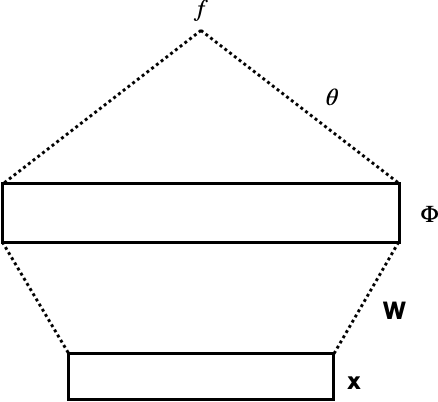
\includegraphics[scale=0.3]{images/nnet.png}
  \caption{A visualization of the said non linear function}
\end{figure}


Where $\theta \in \real^{n \times 1}$, $\textbf{W} \in \real^{n \times p}$ is the weight matrix, and both are the parameters for our non linear model. The feature vector is  $\textbf{x} \in \real^{p \times 1}$. The function $g : \real^{n \times 1} \rightarrow \real^{n \times 1}$ where $g$ an element-wise applied non-linearity e.g. tanh, ReLU.
$\Phi$ is an additional notation to aid in understanding further.
\subsection{SGD and Backpropagation }
Putting the non linear approximation  \ref{eq:non_linear_function} in the SGD equation and optimizing for parameter $\theta_{t+1}$.
\begin{equation}\label{eq:backprop1}
    \begin{split}
        \theta_{t+1} &= \theta_t - \alpha_t \nabla_{\theta_t}(Y_t - f(\textbf{x}_t, \theta_t, \textbf{W}_t))^2\\
        &= \theta_t + 2 \alpha_t (Y_t - \theta^T \Phi_t)\Phi_t\\
    \end{split}
\end{equation}

Optimizing w.r.t. to the Weight matrix $\textbf{W}$
\begin{equation}\label{der:weight_optimization_non_linear}
    \begin{split}
        \textbf{W}_{t+1} &= \textbf{W}_t - \alpha_t \nabla_{\textbf{W}_t}(Y_t - \theta_t^T\Phi)^2\\
        &= \textbf{W}_t + 2\alpha_t (Y_t - \theta_t^T\Phi_t)\nabla_{\textbf{W}_t} (\theta_t^T\Phi_t)\\
        &= \textbf{W}_t + 2\alpha_t (Y_t - \theta_t^T\Phi_t)(\theta_t \circ g'(\textbf{W}_t\textbf{x}_t))\textbf{x}_t^T \text{ (where $\circ$ is the Hadamard Product)}
    \end{split}
\end{equation}
Hence the final equations
\begin{equation}\label{eq:backprop2}
    \textbf{W}_{t+1} = \textbf{W}_t + 2\alpha_t (Y_t - \theta_t^T\Phi_t)(\theta_t \circ g'(\textbf{W}_t\textbf{x}_t))\textbf{x}_t^T
\end{equation}

So Equations \ref{eq:backprop1} and\ref{eq:backprop2} 
 gives us the update rule for the parameters of the Non linear function approximator.
 
 




\bibliographystyle{plain}

\bibliography{reference}

\end{document}

Probably wrong?

\section{Extra}
In this section I try to derive the bias of the least squares solution:
\begin{equation}
	\begin{split}
		\E[Y - \textbf{x}^T\theta]  &= \E[  Y_i - \textbf{x}_i^T (\sum \textbf{x}_i \textbf{x}_i^T)^{-1}(\sum \textbf{x}_i Y_i) ]\\
		& \text{ (taking the conditional expectation over x)}\\
		&= \E_{\textbf{x}} [ \E_{Y|\textbf{x}} [Y_i -  \xvec_i^T(\sum \xvec_i \xvec_i^T)^{-1}(\sum \xvec_i Y_i)] ]\\
		& \text{ (We need to find the bias for each value $
		\xvec$, i.e. bias wont be dependent on the value of $\xvec$,}\\
		& \text{we can calculate the value of bias for each $\xvec$ and can be redefined on $Y|\xvec$)}\\
		&= \E_{Y|\textbf{x}} [Y_i -  \xvec_i^T(\sum \xvec_i \xvec_i^T)^{-1}(\sum \xvec_i Y_i)]\\
		&=  \E[Y]  -  \xvec_1^T(\sum \xvec_1 \xvec_1^T)^{-1}(\sum \xvec_1 \E[Y])\\
		& \text{( over here we are considering for the case where $\xvec = \xvec_1$)}\\
		&= \E[Y](1 -\xvec_1^T(\sum \xvec_1 \xvec_1^T)^{-1}(\sum \xvec_1) )\\
		&= \E[Y](1 -\xvec_1^T(\cancel{n} \xvec_1 \xvec_1^T)^{-1}(\cancel{n}  \xvec_1) )\\
	    Bias &= \E[Y](1 -\xvec_1^T( \xvec_1 \xvec_1^T)^{-1}(  \xvec_1) )\\
	    & \text{(Multiply the both sides on right hand by $\xvec^T$)}\\
	    Bias\xvec_1^T &= \E[Y](\xvec_1^T -\xvec_1^T\cancel{( \xvec_1 \xvec_1^T)}^{-1}\cancel{(  \xvec_1\xvec_1^T )})\\
	    Bias\xvec_1^T &= \E[Y](\cancel{\xvec_1}^T - \cancel{\xvec_1}^T)\\
	    & \text{(this gives us the Bias to be zero)}\\
	    Bias \xvec_1^T = 0
	\end{split}
\end{equation}

If $\xvec^T$ is not zero then $Bias= 0 $.


